\documentclass[12pt,a4paper]{article}
\usepackage[UTF8,fontset=none,heading=true]{ctex}
\setmainfont{Times New Roman}
\setCJKmainfont[Path=/System/Library/Fonts/Supplemental/]{Songti.ttc}
\setCJKsansfont[Path=/System/Library/Fonts/]{STHeiti Medium.ttc}
\setCJKmonofont[Path=/Library/Fonts/]{Arial Unicode.ttf}
\setCJKfamilyfont{hei}[Path=/System/Library/Fonts/]{STHeiti Medium.ttc}
\newcommand{\heiti}{\CJKfamily{hei}}
\usepackage{geometry}
\usepackage{amsmath,amssymb,amsthm}
\usepackage{graphicx}
\usepackage{booktabs}
\usepackage{longtable}
\usepackage{array}
\usepackage{hyperref}
\usepackage{fancyhdr}
\usepackage{xcolor}
\usepackage{listings}
\usepackage{setspace}
\renewcommand{\labelitemi}{}
\renewcommand{\labelitemii}{}
\renewcommand{\labelitemiii}{}
\usepackage{tikz}
\usetikzlibrary{arrows.meta,positioning,shapes.geometric}

\ctexset{
  section = {
    name = {,、},
    number = \chinese{section},
    format = {\Large\bfseries\raggedright}
  }
}

\geometry{left=2.5cm,right=2.5cm,top=2.5cm,bottom=2.5cm}
\setlength{\headheight}{15pt}
\setstretch{1.5}

\pagestyle{fancy}
\fancyhf{}
\fancyhead[C]{发明专利技术交底书}
\fancyfoot[C]{\thepage}

\title{\textbf{发明专利技术交底书} \\[0.5em]
\Large 一种面向异构计算硬件场景的基于张量同构陷门的抗量子数字签名方法、系统、设备及介质}
\author{中国移动通信有限公司研究院}
\date{2026年3月31日}

\begin{document}

\begin{center}
    {\Large\heiti 中国移动专利申请} \\[1em]
    {\Huge\heiti 技术交底书} \\[1em]
    {\large 中国移动通信集团有限公司} \\[1em]
\end{center}

\noindent
\begin{tabular}{|p{3cm}|p{12cm}|}
\hline
公司编号 &  \\
\hline
发明名称 & 一种面向异构计算硬件场景的基于张量同构陷门的抗量子数字签名方法、系统、设备及介质 \\
\hline
申报单位 & 研究院 \\
\hline
申报类型 & 发明 \\
\hline
发明人 & 许达 \\
\hline
技术联系人 & 许达 (xudayj@chinamobile.com, +86-13521894156) \\
\hline
注意事项 & 1．技术联系人应为深入了解本申请提案技术方案的技术人员。 \\
         & 2．请按照集团公司提供的本技术交底书模板逐项填写。 \\
\hline
\end{tabular}

\vspace{1cm}

%==============================================================================
\section{发明名称}
%==============================================================================

一种面向异构计算硬件场景的基于张量同构陷门的抗量子数字签名方法、系统、设备及介质。


%==============================================================================
\section{技术领域}
%==============================================================================

本发明涉及密码学、网络安全、联邦学习安全、智能网联汽车安全以及 AI 设备软件供应链安全领域，特别涉及一种可部署在量子计算网络节点准入认证、AI 加速设备固件升级包签名、模型发布清单完整性校验、跨域联邦学习中模型梯度张量防投毒与显存内原生验签、分布式 AI 训练集群中的梯度/检查点同步验签，以及自动驾驶与车路协同 V2X 高频广播消息验签等场景中的、基于有限域高阶张量同构陷门构造的抗量子数字签名方法、系统、设备及介质。所述异构计算硬件包括但不限于 GPU、NPU、Tensor Core、边缘 AI 加速卡、车载 AI 芯片及可执行有限域矩阵/张量运算的处理器。

对这六个场景来说，本专利特别重要的原因分别是：节点认证场景中，错误节点一旦接入，后续调度和资源分配都会受影响，因此越早拦截越重要；固件升级场景中，一旦装载错误镜像，恢复成本高，因此装载前校验特别重要；模型发布场景中，一个被污染的模型可能被快速同步到多个推理节点，因此发布前校验特别重要；联邦学习场景中，梯度数据量大、轮次多，如果每轮都先搬到 CPU 再验签，会明显拖慢训练，因此显存内原生验签特别重要；分布式 AI 训练集群同步场景中，梯度分片和检查点分片更新非常频繁，如果同步前无法快速验签，就会影响整个训练任务的吞吐量和恢复效率，因此同步链路验签特别重要；自动驾驶和 V2X 场景中，广播消息更新频率高、决策时延要求严，一旦把伪造或篡改消息送进感知和规划链路，后果直接落到物理世界，因此毫秒级入口验签特别重要。

\textbf{关联项目：}\underline{\hspace{8cm}}（待填写）

%==============================================================================
\section{现有技术的技术方案}
%==============================================================================

\subsection{现有后量子签名技术路线}

现有公开的后量子签名方案大多是通用签名工具，并非针对本申请所涉及的六类具体场景量身设计。这些方案可以完成签名功能，但未必适合直接部署到节点准入、固件升级、模型发布、联邦学习聚合、分布式训练同步和 V2X 广播验签流程中。

现有公开研究和工业部署中的后量子签名技术主要包括以下几类：

\begin{enumerate}
    \item \textbf{格密码路线}：典型代表包括 Falcon、Dilithium 等。该类方案通常基于短向量搜索、模块格或 NTRU 结构构造签名，并依赖离散高斯采样、拒绝采样、模约简或傅里叶域运算来实现签名分布控制和安全性约束。
    \item \textbf{哈希路线}：典型代表包括 SPHINCS+。其安全性主要建立在哈希原语之上，优点在于假设简单，但签名或公钥尺寸通常较大，验证吞吐量受限。
    \item \textbf{纠错码路线}：该类方案通常具有较强的抗量子属性，但公钥尺寸较大，难以直接用于带宽敏感型签名场景。
    \item \textbf{多变量路线}：该类方案多基于多变量多项式映射的求逆困难性，但公开历史中已有部分方案在参数设计或代数结构泄露方面被攻破。
    \item \textbf{同源或同构相关路线}：部分方案基于图同构、多项式同构或椭圆曲线同源构造身份识别或签名机制，但在工程上尚未形成适配大规模软件与设备签名的统一方案。
\end{enumerate}

\subsection{现有识别到签名的构造方式}

现有数字签名中还常见一类构造思路，即先构建交互式身份识别协议，再通过 Fiat-Shamir 变换将其转化为非交互式签名。该思路解决的是签名生成的密码学框架问题，但通常不涉及与具体业务流程的结合。该类方法的关键在于：

\begin{itemize}
    \item 需要存在一个难以伪造、但易于由合法持钥人应答的交互式证明关系；
    \item 需要承诺、挑战和响应三者之间满足可公开验证的一致性；
    \item 需要避免在实现中引入过多浮点分支、失败重试或参数敏感逻辑，否则会增加侧信道风险。
\end{itemize}

\subsection{现有技术在工程实现上的共同特点}

现有方案在工程层面的主要问题不在于理论上能否完成签名，而在于实际部署时的性能、复杂度和系统影响。在上述六类实际系统中，现有后量子签名方案大多具有如下工程特征：

\begin{itemize}
    \item 依赖标量或向量级运算，难以直接映射到面向张量收缩优化的 AI 加速硬件，导致在设备侧固件校验、模型批量分发、分布式训练梯度同步以及联邦学习梯度校验场景中难以复用现有张量算力；
    \item 在签名端或验证端经常需要进行噪声控制、范数检查、拒绝采样或近似分布采样，不利于在节点准入控制器、可信启动链、模型仓库校验代理、训练加速卡运行时和车载控制器中构造路径稳定的验证实现；
    \item 对侧信道敏感设备而言，实现常数时间路径较为复杂，特别是在安全启动固件、受限控制面代理以及显存内安全校验链路中部署成本较高；
    \item 多数方案的公钥、签名或计算流程仍围绕低阶线性结构展开，未充分利用高阶张量上的非交换群作用结构，也未将节点身份字段、固件版本字段、模型发布字段、梯度元数据字段、检查点分片字段和 V2X 广播字段合并为统一的场景化签名载荷。
\end{itemize}

%==============================================================================
\section{现有技术的缺点及本申请提案要解决的技术问题}
%==============================================================================

现有技术主要存在以下缺点和技术问题：

(1) \textbf{通用签名接口与实际业务脱节}：现有技术通常将消息当作任意比特串处理，但真实系统中需要校验的是节点身份字段、固件版本信息、模型摘要、联邦学习梯度元数据、分布式训练检查点分片信息以及 V2X 广播信标字段等具有明确语义的结构化数据。现有方案未将这些字段作为原生对象纳入设计，导致工程结合度不高。

(2) \textbf{现有后量子签名实现复杂}：以 Falcon 为代表的紧凑型格签名方案通常需要离散高斯采样、浮点近似、拒绝采样或复杂的范数控制逻辑。这类流程理论上可行，但工程实现复杂度较高，部署到节点准入、升级校验、训练同步链路或 V2X 运行时中时维护成本较高。

(3) \textbf{稳定实现难度较大}：当签名算法依赖浮点运算、条件分支和重试机制时，程序运行路径更不稳定。在安全启动链、固件升级代理、训练集群同步运行时以及联邦学习显存侧验签链路中，这类不稳定路径会增加实现难度。

(4) \textbf{大规模部署时容易出现实现敏感性问题}：部分现有方案在参数边界、采样近似误差或编码处理不当时，可能出现失败重试或实现差异放大的问题。这类问题在小规模测试中不一定突出，但在大规模节点认证、批量固件校验、模型分发、训练集群同步和联邦学习更新场景中会被放大。

(5) \textbf{未充分利用现有 AI 硬件}：当前 GPU、NPU、Tensor Core 等硬件擅长张量计算，但多数现有签名方案并非围绕张量原语构造，因此难以直接复用这些硬件优势。该问题在联邦学习场景中尤其突出，因为待校验对象本身即为张量。

(6) \textbf{缺少一种能统一覆盖这六类场景的方案}：现有公开技术中，尚缺少一种既是抗量子的，又能把节点准入、固件升级、模型发布、联邦学习梯度校验、分布式训练同步验签和 V2X 高频广播验签统一起来的工程方案。

基于上述问题，本申请拟解决以下技术问题：提供一种适合直接部署到真实系统中的抗量子签名方案。该方案不依赖格噪声、高斯采样和复杂重试流程，而是在有限域上通过矩阵乘法和张量收缩完成密钥生成、签名与验证；同时将节点认证报文、固件升级清单、模型发布清单、联邦学习梯度载荷、分布式训练检查点/梯度分片载荷以及 V2X 广播载荷直接作为签名保护对象，使验签结果可直接用于业务流程的放行或阻断决策。在联邦学习和分布式训练场景中，本申请重点解决的问题是：避免将大量张量数据搬运到 CPU 侧进行验签，而是直接在 GPU/NPU 显存或张量计算链路中完成验签；在 V2X 场景中，本申请重点解决的问题是：在毫秒级处理预算内完成高频广播消息的快速验签。

更具体地，本申请方案期望达到以下直接技术效果：
\begin{itemize}
    \item 非法节点想加入量子计算网络时，可以在接入前被拦住；
    \item 不匹配型号、被回退版本或被篡改的固件镜像，可以在装载前被拦住；
    \item 被污染的模型文件或依赖清单，可以在发布前被拦住；
    \item 来历异常或被篡改的梯度更新，可以在进入联邦聚合前被拦住；
    \item 来历异常或被篡改的梯度分片、检查点分片和参数同步块，可以在进入训练同步链路前被拦住；
    \item 被伪造或被篡改的 V2X 广播消息，可以在进入车端决策链路前被拦住。
\end{itemize}

%==============================================================================
\section{本申请提案的技术方案的详细阐述}
%==============================================================================

本申请提出一种 TITAN（Tensor Isomorphism Trapdoor Asymmetric Network，张量同构陷门非对称网络）抗量子数字签名方案。本方案的核心在于：

\textbf{构建一套能直接嵌入节点接入、固件升级、模型发布、联邦学习聚合、分布式训练同步和 V2X 广播验签流程中的签名校验机制，而非脱离业务场景的通用签名算法。}

其核心设计思路包括三个方面：
\begin{itemize}
    \item 利用张量同构关系构造公钥和私钥之间的对应关系；
    \item 采用统一的签名和验签流程处理六类不同业务对象；
    \item 使验签结果直接控制业务系统的放行或阻断动作。
\end{itemize}

在实现上，该方案部署在异构计算硬件边界上，部署位置包括量子计算网络节点准入控制器、AI 加速设备可信启动/升级代理、模型仓库发布校验代理、联邦学习训练加速卡运行时、分布式训练集群同步代理以及车端 V2X 消息验签模块。其核心基于有限域 $\mathbb{F}_p$ 上三阶张量的模态群作用关系构造公私钥陷门，并通过多轮承诺、挑战和响应关系，经 Fiat-Shamir 变换得到非交互数字签名，使六类业务载荷都以统一但场景化的方式进入签名与验证流程。

\subsection{基本数学对象}

这一小节先说明本专利最底层的“数学骨架”。评审人在这里需要抓住一个直观认识：本方案不是靠浮点采样或复杂噪声控制来做签名，而是把核心运算统一成有限域上的矩阵乘法和张量变换，这样更容易落到现有 GPU、NPU 等硬件上。

设有限域为 $\mathbb{F}_p$，其中 $p$ 为素数；设张量维度为 $N$；设公开基准张量为
\[
\mathcal{T}_0 \in \mathbb{F}_p^{N \times N \times N}.
\]

定义三个模态上的张量作用为：
\[
\mathcal{T}' = \mathcal{T} \times_1 A \times_2 B \times_3 C,
\]
其中 $A,B,C \in \mathbb{F}_p^{N \times N}$，且
\[
\mathcal{T}'(i,j,k)=\sum_{x=1}^{N}\sum_{y=1}^{N}\sum_{z=1}^{N}
A_{i,x}B_{j,y}C_{k,z}\mathcal{T}(x,y,z)\pmod p.
\]

在本申请中，私钥对应于三个可逆矩阵
\[
U,V,W \in GL(N,\mathbb{F}_p),
\]
公钥由上述三个矩阵作用于基准张量得到：
\[
\mathcal{T}_{pk}=\mathcal{T}_0 \times_1 U \times_2 V \times_3 W.
\]

\subsection{系统组成}

从工程实现角度看，本专利不是单独的数学公式，而是一套可以装进真实系统里的模块化方案。评审人可以把它理解为：前面负责准备参数和密钥，中间负责生成签名，后面负责在业务入口做验签，并把验签结果直接交给放行或阻断模块。

本申请的系统可包括如下功能模块：

\begin{itemize}
    \item \textbf{参数生成模块}：用于生成有限域参数 $p$、张量维度 $N$、签名轮数 $r$、哈希函数 $H$ 及公开基准张量 $\mathcal{T}_0$；
    \item \textbf{密钥生成模块}：用于生成三个私钥矩阵 $U,V,W$ 及公钥张量 $\mathcal{T}_{pk}$；
    \item \textbf{承诺生成模块}：用于针对待签名的节点认证报文、固件升级清单、模型发布清单、联邦学习梯度载荷、训练同步清单或 V2X 广播载荷生成随机掩码矩阵和临时承诺张量；
    \item \textbf{挑战派生模块}：用于根据结构化业务载荷和承诺张量计算哈希摘要并导出挑战序列；
    \item \textbf{响应生成模块}：用于根据挑战位选择输出原始掩码矩阵或隐身重构矩阵；
    \item \textbf{签名验证模块}：用于在节点准入控制器、设备安全启动链/升级代理、模型仓库校验代理、联邦学习聚合运行时、训练同步代理或车端消息验签模块处，基于公开基准张量或公钥张量重构承诺并校验摘要一致性；
    \item \textbf{硬件加速模块}：可选地部署于 GPU、NPU、FPGA 或支持张量乘加的处理器上，以实现矩阵乘法和张量收缩的并行计算。
\end{itemize}

上述模块之间的协同关系如图 1 所示。图 1 展示了公开参数、密钥生成、签名生成、签名验证以及硬件加速支撑之间的对应关系，用于说明本申请的系统构成。

\begin{figure}[htbp]
    \centering
    \resizebox{0.94\textwidth}{!}{%
    \begin{tikzpicture}[
        font=\small,
        node distance=11mm and 9mm,
        module/.style={draw, rounded corners=2pt, align=center, minimum width=32mm, minimum height=9mm, fill=gray!8},
        data/.style={draw, trapezium, trapezium left angle=70, trapezium right angle=110, align=center, minimum width=30mm, minimum height=9mm, fill=blue!8},
        accel/.style={draw, rounded corners=2pt, align=center, text width=104mm, minimum height=12mm, inner ysep=2.5mm, fill=green!8},
        line/.style={-Latex, thick}
    ]
        \node[data] (param) {公开参数\\$p,N,r,H,\mathcal{T}_0$};
        \node[module, right=of param] (keygen) {密钥生成模块\\生成 $U,V,W,\mathcal{T}_{pk}$};
        \node[module, below=of keygen] (commit) {承诺生成模块\\生成 $\mathcal{C}^{(t)}$};
        \node[module, left=of commit] (inputmsg) {输入消息\\$M$};
        \node[module, right=of commit] (challenge) {挑战派生模块\\计算 $\rho,c_t$};
        \node[module, below=of challenge] (response) {响应生成模块\\输出 $S^{(t)}$};
        \node[module, left=of response] (package) {签名封装\\形成 $\sigma$};
        \node[module, right=of response] (verify) {签名验证模块\\校验 $\rho'=\rho$};
        \node[accel, below=22mm of commit] (accel) {硬件加速模块（GPU/NPU/FPGA/Tensor Core）\\支持矩阵乘法、有限域求逆和张量收缩计算};

        \draw[line] (param) -- (keygen);
        \draw[line] (param) -- (commit);
        \draw[line] (param.east) |- (verify.north);
        \draw[line] (keygen) -- (commit);
        \draw[line] (keygen) -- (verify);
        \draw[line] (inputmsg) -- (challenge);
        \draw[line] (commit) -- (challenge);
        \draw[line] (challenge) -- (response);
        \draw[line] (response) -- (package);
        \draw[line] (package) -- (verify);

        \draw[line, dashed] (accel.north) -- (commit.south);
        \draw[line, dashed] (accel.north west) -- ++(0,9mm) -| (keygen.south);
        \draw[line, dashed] (accel.north east) -- ++(0,9mm) -| (verify.south);
    \end{tikzpicture}
    }
    \caption{TITAN 抗量子签名系统架构图}
\end{figure}

\subsection{部署形态说明}

这一小节回答“这套方案具体装在哪里、什么时候触发”。简化理解就是：谁负责接入控制，谁负责升级装载，谁负责模型发布，谁负责联邦学习聚合，谁负责训练同步，谁负责车端广播消息入口，谁就在自己的入口位置调用本专利的验签能力。评审人在这里可以直接把本方案理解为“部署在各类业务入口上的签名门禁”。

本申请的技术方案在不同场景中具有差异化的部署形态：

(1) 在方法层面，由节点准入控制器、设备安全启动链/升级代理、模型仓库校验代理、联邦学习计算图运行时、分布式训练同步代理和车端 V2X 消息验签模块执行结构化数据采集、签名生成、签名验证及阻断处置步骤。

(2) 在系统层面，由处理器、存储器、总线接口、密钥存储区、张量运算模块、验证控制模块和策略执行模块组成，用于完成前述签名和校验动作。

(3) 在存储介质层面，在非暂态计算机可读存储介质上存储程序指令，所述程序指令在被处理器执行时，使设备完成前述方法步骤。

在一个实施例中，节点准入控制器从接入报文缓冲区读取节点证书摘要、节点角色、调度域和握手随机数，处理器完成结构化载荷编码后调用张量验签模块，验签结果再传递给准入策略模块，以控制是否允许节点加入量子计算网络；在另一实施例中，设备安全启动链从镜像头部读取设备型号、固件版本、镜像哈希和回滚计数器，验签通过后才允许镜像装载；在又一实施例中，模型仓库校验代理读取模型权重摘要、依赖清单摘要和目标加速器型号，验签通过后才允许模型发布或下载；在第四实施例中，联邦学习中的梯度张量或模型更新块驻留于 GPU/NPU 显存中，验签过程在不跨越主机总线的情况下完成，再决定是否允许该更新进入聚合器；在第五实施例中，分布式训练集群的同步代理在发送或接收梯度分片、参数块或检查点分片时，直接调用张量验签模块，验签通过后才允许该数据进入 all-reduce、参数恢复或断点续训流程；在第六实施例中，车端 V2X 消息验签模块在接收到周边车辆或路侧单元发来的广播信标后，先校验消息中的时间戳、位置字段、速度字段和事件标签，再决定是否将该广播送入感知融合和轨迹规划链路。

\subsection{密钥生成方法}

这一部分对应“先把钥匙配好”。也就是说，系统先生成一组只有签名方自己掌握的私钥矩阵，再由此推出公开给验证方使用的公钥张量，后续签名和验签都围绕这组关系展开。

\subsubsection{1. 公开参数初始化}

参数生成模块选定素数 $p$、张量阶数和维度 $N$、签名轮数 $r$ 以及哈希函数 $H$。公开基准张量 $\mathcal{T}_0$ 可以直接存储，也可以通过公开种子经确定性扩展算法生成，以降低参数分发开销。

\subsubsection{2. 私钥生成}

密钥生成模块随机生成三个满秩可逆矩阵 $U,V,W$。为便于嵌入式实现，矩阵既可采用一般稠密矩阵形式，也可采用块对角、循环、Toeplitz 或种子展开的结构化形式。

\subsubsection{3. 公钥生成}

根据私钥矩阵计算公钥张量：
\[
\mathcal{T}_{pk}=\mathcal{T}_0 \times_1 U \times_2 V \times_3 W.
\]

在一个实施例中，当 $N=10,p=251$ 时，若按每个张量元素使用 1 字节编码，则公钥张量主体数据量为 $10 \times 10 \times 10=1000$ 字节。

\subsection{签名生成方法}

这一部分回答“签名到底怎么生成”。直观上看，就是先针对业务载荷生成一批临时承诺，再根据消息内容导出挑战，最后按挑战输出相应的响应数据，组合成可验证的签名。

在本申请中，待签名对象 $M$ 不是脱离应用场景的任意比特串，而是由业务系统按预定字段顺序序列化得到的结构化载荷。在不同实施例中，$M$ 可分别取为：量子计算网络节点认证报文 $M_{node}$，其至少包括节点身份证书摘要、节点角色、调度域标识、会话时间戳和握手随机数；AI 加速设备固件升级清单 $M_{fw}$，其至少包括设备型号、固件版本号、镜像哈希、回滚计数器和发布时间戳；模型发布清单 $M_{model}$，其至少包括模型权重哈希、推理框架版本、目标加速器型号、依赖包摘要和发布版本号；联邦学习梯度载荷 $M_{fl}$，其至少包括轮次号、梯度张量摘要、参与节点标识、训练任务编号和目标模型版本；分布式训练同步载荷 $M_{sync}$，其至少包括训练步号、梯度分片摘要、检查点分片编号、作业标识和目标模型版本；V2X 广播载荷 $M_{v2x}$，其至少包括消息时间戳、车辆或路侧单元标识、位置字段、速度字段、事件标签和消息序号。验证端仅当相应业务字段校验通过时才进入签名验证流程，因此签名对象的组织方式、验证入口和业务动作三者不可分离。

设待签名消息为 $M$，签名轮数为 $r$。

\subsubsection{1. 承诺阶段}

对于每一轮 $t\in\{1,\dots,r\}$，签名者随机生成三个可逆掩码矩阵
\[
R_A^{(t)},R_B^{(t)},R_C^{(t)} \in GL(N,\mathbb{F}_p),
\]
并计算临时承诺张量
\[
\mathcal{C}^{(t)}=\mathcal{T}_0 \times_1 R_A^{(t)} \times_2 R_B^{(t)} \times_3 R_C^{(t)}.
\]

\subsubsection{2. 挑战阶段}

将消息和所有承诺张量串接后输入哈希函数：
\[
\rho = H\big(M \parallel \mathcal{C}^{(1)} \parallel \cdots \parallel \mathcal{C}^{(r)}\big).
\]

再由摘要 $\rho$ 按位或按分组导出挑战序列
\[
c_1,c_2,\dots,c_r.
\]
在一个实施方式中，$c_t \in \{0,1\}$。

\subsubsection{3. 响应阶段}

设 $U^{-1},V^{-1},W^{-1}$ 为私钥矩阵在 $\mathbb{F}_p$ 上的逆矩阵。对于第 $t$ 轮：

\begin{itemize}
    \item 若 $c_t=0$，则输出原始掩码矩阵
    \[
    S^{(t)}=\big(R_A^{(t)},R_B^{(t)},R_C^{(t)}\big);
    \]
    \item 若 $c_t=1$，则输出隐身重构矩阵
    \[
    Z_A^{(t)}=R_A^{(t)}U^{-1},\quad
    Z_B^{(t)}=R_B^{(t)}V^{-1},\quad
    Z_C^{(t)}=R_C^{(t)}W^{-1},
    \]
    并令
    \[
    S^{(t)}=\big(Z_A^{(t)},Z_B^{(t)},Z_C^{(t)}\big).
    \]
\end{itemize}

最终签名为
\[
\sigma=\big(\rho,S^{(1)},S^{(2)},\dots,S^{(r)}\big).
\]

\subsection{签名验证方法}

这一部分回答“验证方如何快速判断真假”。对评审人来说，最关键的是看明白两点：第一，验证时不需要知道私钥；第二，验证通过后不是只输出一个数学结果，而是直接决定是否接入、是否装载、是否发布、是否允许梯度进入聚合。

验证者输入消息 $M$、签名 $\sigma$ 以及公钥 $\mathcal{T}_{pk}$ 后，执行如下步骤。对应到具体部署场景时，节点准入控制器接收 $M_{node}$ 并在节点接入前完成验证；设备安全启动链或升级代理接收 $M_{fw}$ 并在装载镜像前完成验证；模型仓库校验代理接收 $M_{model}$ 并在模型分发或加载前完成验证；联邦学习聚合器或本地训练运行时接收 $M_{fl}$ 并在参数聚合前完成验证；分布式训练同步代理接收 $M_{sync}$ 并在参数同步或断点恢复前完成验证；车端 V2X 消息验签模块接收 $M_{v2x}$ 并在广播消息进入感知融合或规划模块前完成验证。若结构化字段中存在设备型号不匹配、版本号回退、依赖摘要不一致、任务编号冲突、模型版本异常、检查点分片编号异常或消息时间戳失配等业务异常，则系统可直接阻断后续流程。

\subsubsection{1. 解析挑战}

验证者根据签名中的摘要 $\rho$ 导出挑战序列 $c_1,\dots,c_r$。

\subsubsection{2. 重构承诺}

对于每一轮 $t$：

\begin{itemize}
    \item 当 $c_t=0$ 时，验证者利用公开基准张量重构
    \[
    \widehat{\mathcal{C}}^{(t)}=\mathcal{T}_0 \times_1 R_A^{(t)} \times_2 R_B^{(t)} \times_3 R_C^{(t)};
    \]
    \item 当 $c_t=1$ 时，验证者利用公钥张量重构
    \[
    \widehat{\mathcal{C}}^{(t)}=\mathcal{T}_{pk} \times_1 Z_A^{(t)} \times_2 Z_B^{(t)} \times_3 Z_C^{(t)}.
    \]
\end{itemize}

由于
\[
\mathcal{T}_{pk}=\mathcal{T}_0 \times_1 U \times_2 V \times_3 W,
\]
因此当 $c_t=1$ 时，有
\[
\widehat{\mathcal{C}}^{(t)}
=\mathcal{T}_0 \times_1 U \times_2 V \times_3 W
\times_1 \big(R_A^{(t)}U^{-1}\big)
\times_2 \big(R_B^{(t)}V^{-1}\big)
\times_3 \big(R_C^{(t)}W^{-1}\big)
=\mathcal{T}_0 \times_1 R_A^{(t)} \times_2 R_B^{(t)} \times_3 R_C^{(t)}.
\]

即，不论挑战位为何值，合法签名者均可使验证端重构出同一承诺张量。

\subsubsection{3. 一致性校验}

验证者重新计算
\[
\rho' = H\big(M \parallel \widehat{\mathcal{C}}^{(1)} \parallel \cdots \parallel \widehat{\mathcal{C}}^{(r)}\big).
\]
若 $\rho'=\rho$，则验证通过；否则验证失败。

本申请的签名生成与验证主流程如图 2 所示。图 2 重点展示了“承诺-挑战-响应”和“基于 $\mathcal{T}_0$ 或 $\mathcal{T}_{pk}$ 的双路径验证”这两个便于理解本申请的关键动作。

\begin{figure}[htbp]
    \centering
    \begin{tikzpicture}[
        font=\small,
        node distance=8mm and 12mm,
        flow/.style={draw, rounded corners=2pt, align=center, minimum width=34mm, minimum height=9mm, fill=gray!8},
        decision/.style={draw, diamond, aspect=2.0, align=center, inner sep=1pt, minimum width=22mm, minimum height=10mm, fill=orange!10},
        term/.style={draw, rounded corners=6pt, align=center, minimum width=30mm, minimum height=9mm, fill=blue!8},
        line/.style={-Latex, thick}
    ]
        \node[term] (start) {输入 $M$、私钥和公钥};
        \node[flow, below=of start] (mask) {按轮生成\\$R_A^{(t)},R_B^{(t)},R_C^{(t)}$};
        \node[flow, below=of mask] (commit2) {计算承诺张量\\$\mathcal{C}^{(t)}$};
        \node[flow, below=of commit2] (hash) {计算摘要 $\rho$\\并导出挑战 $c_t$};
        \node[decision, below=of hash] (chal1) {$c_t=0$?};
        \node[flow, below left=of chal1] (resp0) {输出原始掩码\\$(R_A^{(t)},R_B^{(t)},R_C^{(t)})$};
        \node[flow, below right=of chal1] (resp1) {输出隐身重构矩阵\\$(Z_A^{(t)},Z_B^{(t)},Z_C^{(t)})$};
        \node[flow, below=16mm of chal1] (sigma) {组合得到签名\\$\sigma=(\rho,S^{(1)},\dots,S^{(r)})$};
        \node[flow, below=of sigma] (parse) {验证端解析 $\rho$\\并恢复挑战序列};
        \node[decision, below=of parse] (chal2) {$c_t=0$?};
        \node[flow, below left=of chal2] (ver0) {利用 $\mathcal{T}_0$\\重构 $\widehat{\mathcal{C}}^{(t)}$};
        \node[flow, below right=of chal2] (ver1) {利用 $\mathcal{T}_{pk}$\\重构 $\widehat{\mathcal{C}}^{(t)}$};
        \node[flow, below=16mm of chal2] (rehash) {重算 $\rho'$ 并比较\\$\rho'=\rho$};
        \node[term, below=of rehash] (end) {输出验证通过/失败};

        \draw[line] (start) -- (mask);
        \draw[line] (mask) -- (commit2);
        \draw[line] (commit2) -- (hash);
        \draw[line] (hash) -- (chal1);
        \draw[line] (chal1) -- node[left] {\scriptsize 是} (resp0);
        \draw[line] (chal1) -- node[right] {\scriptsize 否} (resp1);
        \draw[line] (resp0) |- (sigma);
        \draw[line] (resp1) |- (sigma);
        \draw[line] (sigma) -- (parse);
        \draw[line] (parse) -- (chal2);
        \draw[line] (chal2) -- node[left] {\scriptsize 是} (ver0);
        \draw[line] (chal2) -- node[right] {\scriptsize 否} (ver1);
        \draw[line] (ver0) |- (rehash);
        \draw[line] (ver1) |- (rehash);
        \draw[line] (rehash) -- (end);
    \end{tikzpicture}
    \caption{TITAN 抗量子签名生成与验证流程图}
\end{figure}

\subsection{联邦学习场景下的显存内原生验签机制}

本小节重点阐述联邦学习场景下的显存内原生验签机制。

这一场景是本专利特别关键的应用方向。原因在于，联邦学习里传输和聚合的对象本身就是梯度张量，而本专利的签名验证核心也是张量运算，底层硬件又正好是 GPU/NPU 的张量计算单元，因此三者天然对齐，能够把“安全校验”直接并入“训练计算流”。

在跨域联邦学习场景中，待签名对象 $M_{fl}$ 不是普通字符串，而是边缘节点计算出的高维模型梯度张量或模型更新块。现有签名算法通常需要将这些数据从 AI 加速器显存搬运到主机 CPU 内存，再进行哈希和验签。由于梯度数据量较大，这种跨总线搬运会显著降低系统吞吐量。

针对上述问题，本申请提供如下解决方案：\textbf{将验签过程保留在显存中完成，避免梯度数据的跨总线搬运。}

具体地，可将本申请的张量同构验签逻辑直接编译为深度学习框架的自定义算子，并嵌入联邦学习聚合计算流图中。这样，聚合节点在接收到梯度张量后，无需先把梯度拷贝到 CPU 侧内存，而是直接在 GPU、NPU 或 Tensor Core 对应的显存内部完成多轮挑战下的张量重构与一致性校验。校验通过后，流图继续执行聚合函数；校验失败时，异常梯度张量在显存侧直接被阻断，不进入参数聚合过程。

换言之，\textbf{训练用的张量留在原来的地方，安全校验也在原来的地方做完。}

在一个更具体的实施方式中，联邦学习系统可将
\[
\mathcal{T}_{pk}\times_{1}Z_{A}^{(t)}\times_{2}Z_{B}^{(t)}\times_{3}Z_{C}^{(t)}
\]
这一重构过程映射为张量计算核心可直接调度的算子序列，从而复用 AI 芯片原有的矩阵乘法和张量收缩能力。由于待保护对象本身是张量、签名验证核心运算也是张量运算、执行硬件同样面向张量计算进行优化，因此该实施方式实现了“业务计算流”和“安全校验流”的统一。与需要先搬运数据再验签的方案相比，本申请能够减少跨总线搬运、降低 CPU 介入程度，并提升大规模联邦学习场景下的整体吞吐量。

\subsection{真实数值试验与定量结果}

这一小节的目的，是让评审人快速看到本专利不是停留在纸面上的抽象方案，而是已经可以跑起来，并且能给出可量化的结果。这里重点关注三类问题：能不能稳定验签、遇到篡改能不能拦住、放到真实工程入口后大概需要多少时间成本。

为进一步说明本申请方案并非脱离业务系统的抽象算法，而是能够嵌入异构计算硬件上的多种工程流程，本申请开展了真实运行试验，并将原始结果保存在随附实验目录中。相关基础数据全部由实际代码执行得到，不使用模拟数据、插值数据或手工补齐数据。实验程序位于 \path{experiments/run_real_benchmarks.py}，其统一采用 64 字节待签名载荷进行测试；该测试口径对应于将节点认证字段、固件清单字段、模型发布字段、联邦学习梯度元数据字段、训练同步分片字段或 V2X 广播元数据字段完成规范化编码后再进行摘要或序列化的工程输入方式。原始逐次测量结果位于 \path{experiments/results/raw_benchmark.csv}，汇总统计结果位于 \path{experiments/results/summary.json}。

本组实验在同一台机器、同一 Python 运行环境下同时运行 TITAN 原型实现和 Falcon 本地实现，以保证工程比较口径一致。实验环境包括：Windows 11 64 位、Python 3.13.5、NumPy 2.1.3、SymPy 1.14.0。Falcon 对比实现采用本地现有目录中的真实实现代码。需要说明的是，表中 TITAN 参数点用于工程样机验证，尚未映射到与 Falcon 完全一致的标准安全等级，因此以下结果用于说明六类具体部署场景中的共性实现趋势、验证预算和可部署性证据，而非宣称已完成标准安全等级对齐。其中，联邦学习场景的“显存内原生验签”、分布式训练同步场景的“训练链路内验签”以及 V2X 场景的“高频广播快速验签”属于基于相同底层验签算子、相同测得验证时延和相同张量硬件映射逻辑所作的工程实现分析，不额外宣称已完成超大规模集群实网测试或整车道路测试。

\textbf{正确性与篡改拒绝结果}

\begin{table}[htbp]
    \centering
    \small
    \resizebox{\textwidth}{!}{%
    \begin{tabular}{|l|c|c|c|}
        \hline
        方案 & 原始签名验证成功率 & 篡改消息拒绝率 & 篡改签名拒绝率 \\
        \hline
        TITAN N=8, rounds=16 & 50/50 (100\%) & 50/50 (100\%) & 50/50 (100\%) \\
        \hline
        TITAN N=8, rounds=32 & 50/50 (100\%) & 50/50 (100\%) & 50/50 (100\%) \\
        \hline
        TITAN N=10, rounds=32 & 50/50 (100\%) & 50/50 (100\%) & 50/50 (100\%) \\
        \hline
        TITAN N=12, rounds=32 & 50/50 (100\%) & 50/50 (100\%) & 50/50 (100\%) \\
        \hline
        Falcon-512 & 50/50 (100\%) & 50/50 (100\%) & 50/50 (100\%) \\
        \hline
        Falcon-1024 & 50/50 (100\%) & 50/50 (100\%) & 50/50 (100\%) \\
        \hline
    \end{tabular}}
    \caption{真实运行下的正确性与篡改拒绝结果}
\end{table}

表 1 表明：在本次实际执行的 200 次 TITAN 验证试验中，未观察到签名验证失败；且对消息篡改和签名篡改均实现了 100\% 的拒绝。该结果可直接对应到六类业务入口的最基本安全动作：节点准入控制器可据此拒绝被篡改的节点认证报文，设备升级代理可据此拒绝被替换或被回退的固件清单，模型仓库校验代理可据此拒绝被污染的模型发布清单，联邦学习聚合器可据此拒绝被投毒的梯度更新，训练同步代理可据此拒绝异常梯度分片或检查点分片，车端消息验签模块可据此拒绝伪造或被篡改的 V2X 广播消息。换言之，本申请的真实试验已经覆盖“正确载荷可通过、篡改载荷被拒绝”这一场景化部署所必需的核心判定逻辑。

\textbf{与 Falcon 实现的工程指标比较}

\begin{table}[htbp]
    \centering
    \small
    \resizebox{\textwidth}{!}{%
    \begin{tabular}{|l|c|c|c|c|c|c|}
        \hline
        方案 & 公钥字节数 & 私钥字节数 & 签名字节数 & KeyGen均值(ms) & Sign均值(ms) & Verify均值(ms) \\
        \hline
        TITAN N=8, rounds=16 & 512 & 384 & 3104 & 4.539 & 16.534 & 1.808 \\
        \hline
        TITAN N=8, rounds=32 & 512 & 384 & 6176 & 4.936 & 33.794 & 3.495 \\
        \hline
        TITAN N=10, rounds=32 & 1000 & 600 & 9632 & 6.525 & 43.297 & 4.136 \\
        \hline
        TITAN N=12, rounds=32 & 1728 & 864 & 13856 & 10.096 & 50.150 & 4.806 \\
        \hline
        Falcon-512 & 896 & 3584 & 666 & 2328.044 & 16.280 & 4.263 \\
        \hline
        Falcon-1024 & 1792 & 7168 & 1280 & 11414.624 & 40.760 & 10.706 \\
        \hline
    \end{tabular}}
    \caption{TITAN 与 Falcon 的真实工程指标对比}
\end{table}

为直观展示“时间成本”和“尺寸成本”的整体差异，依据同一份真实汇总文件自动生成了图 3 和图 4。图中全部柱状值均来自 \path{experiments/results/summary.json}，未进行手工修饰。

\begin{figure}[htbp]
    \centering
    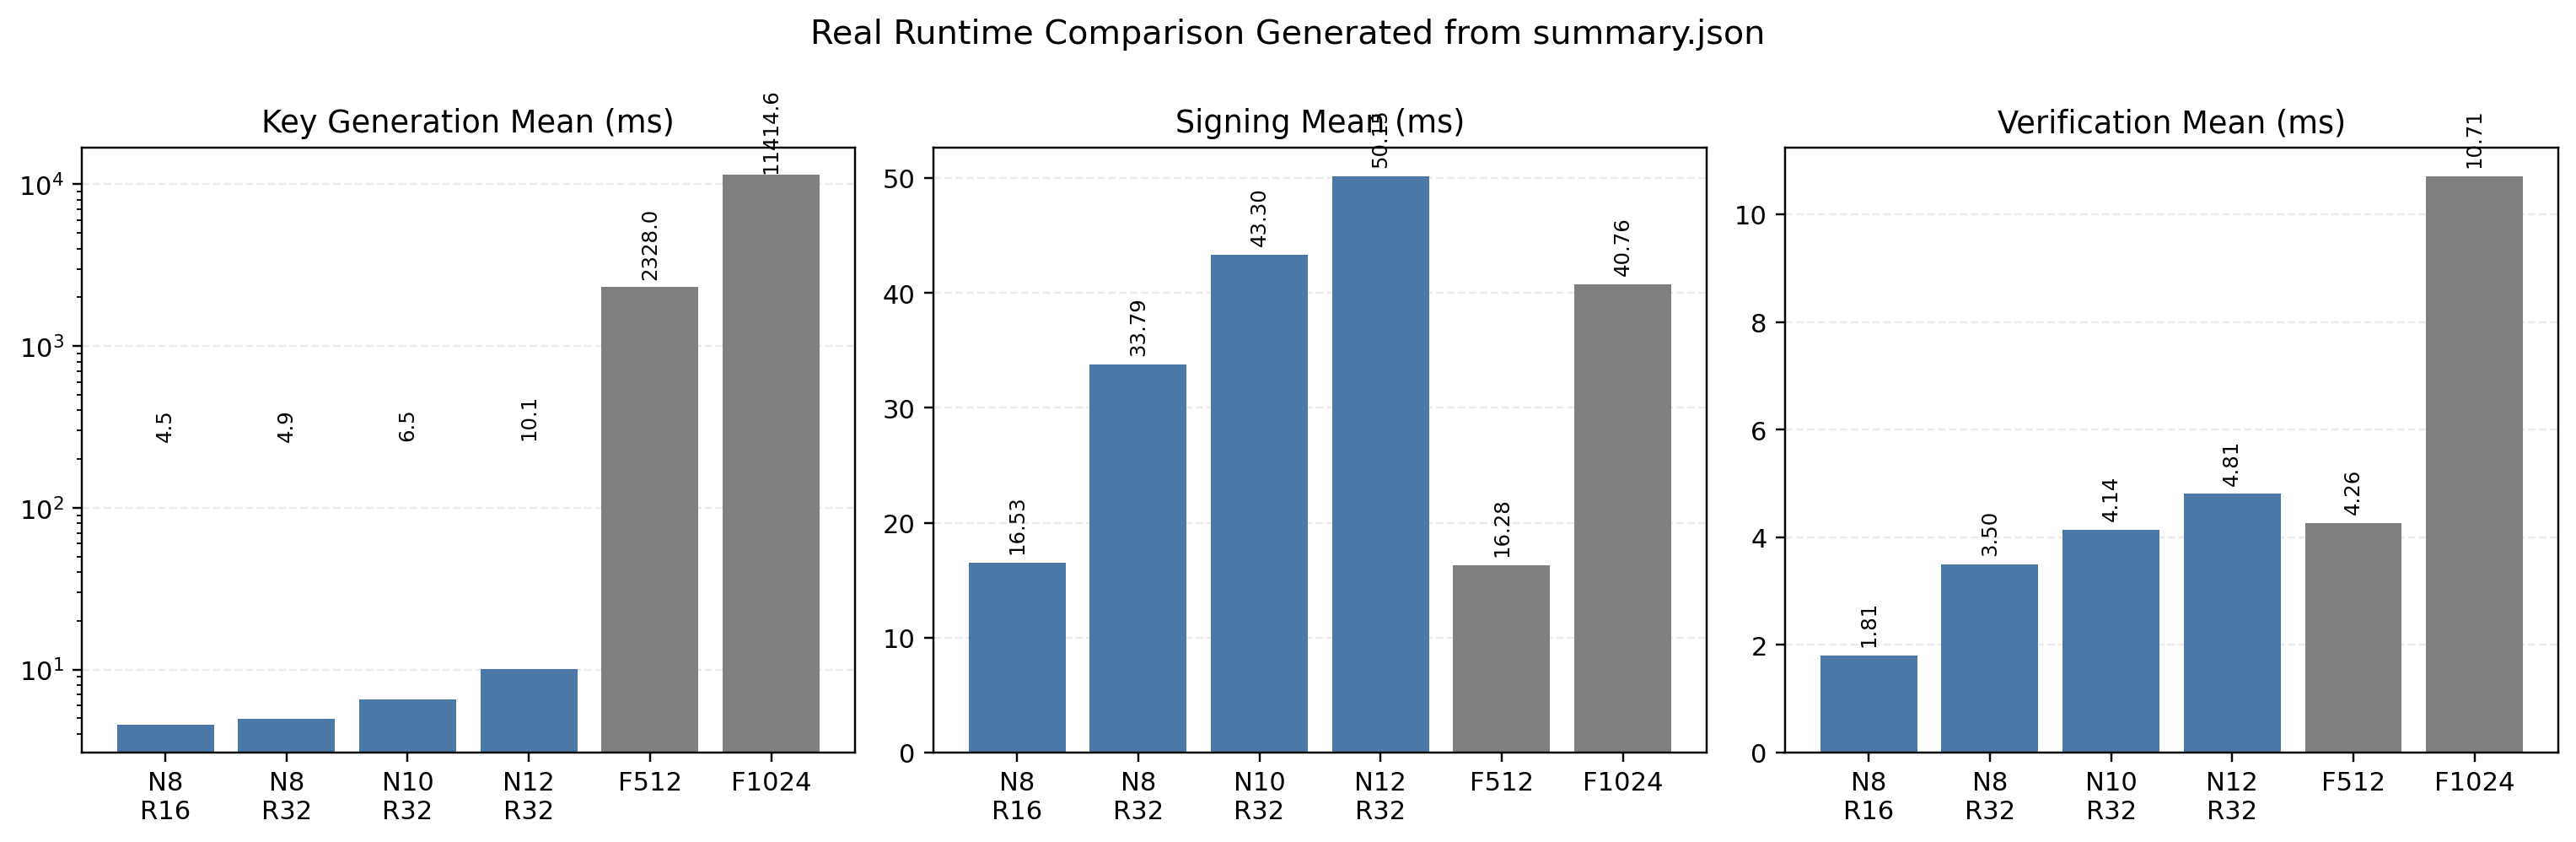
\includegraphics[width=\textwidth]{../experiments/results/latency_comparison.png}
    \caption{基于真实运行结果自动生成的 TITAN 与 Falcon 时间开销对比图}
\end{figure}

\begin{figure}[htbp]
    \centering
    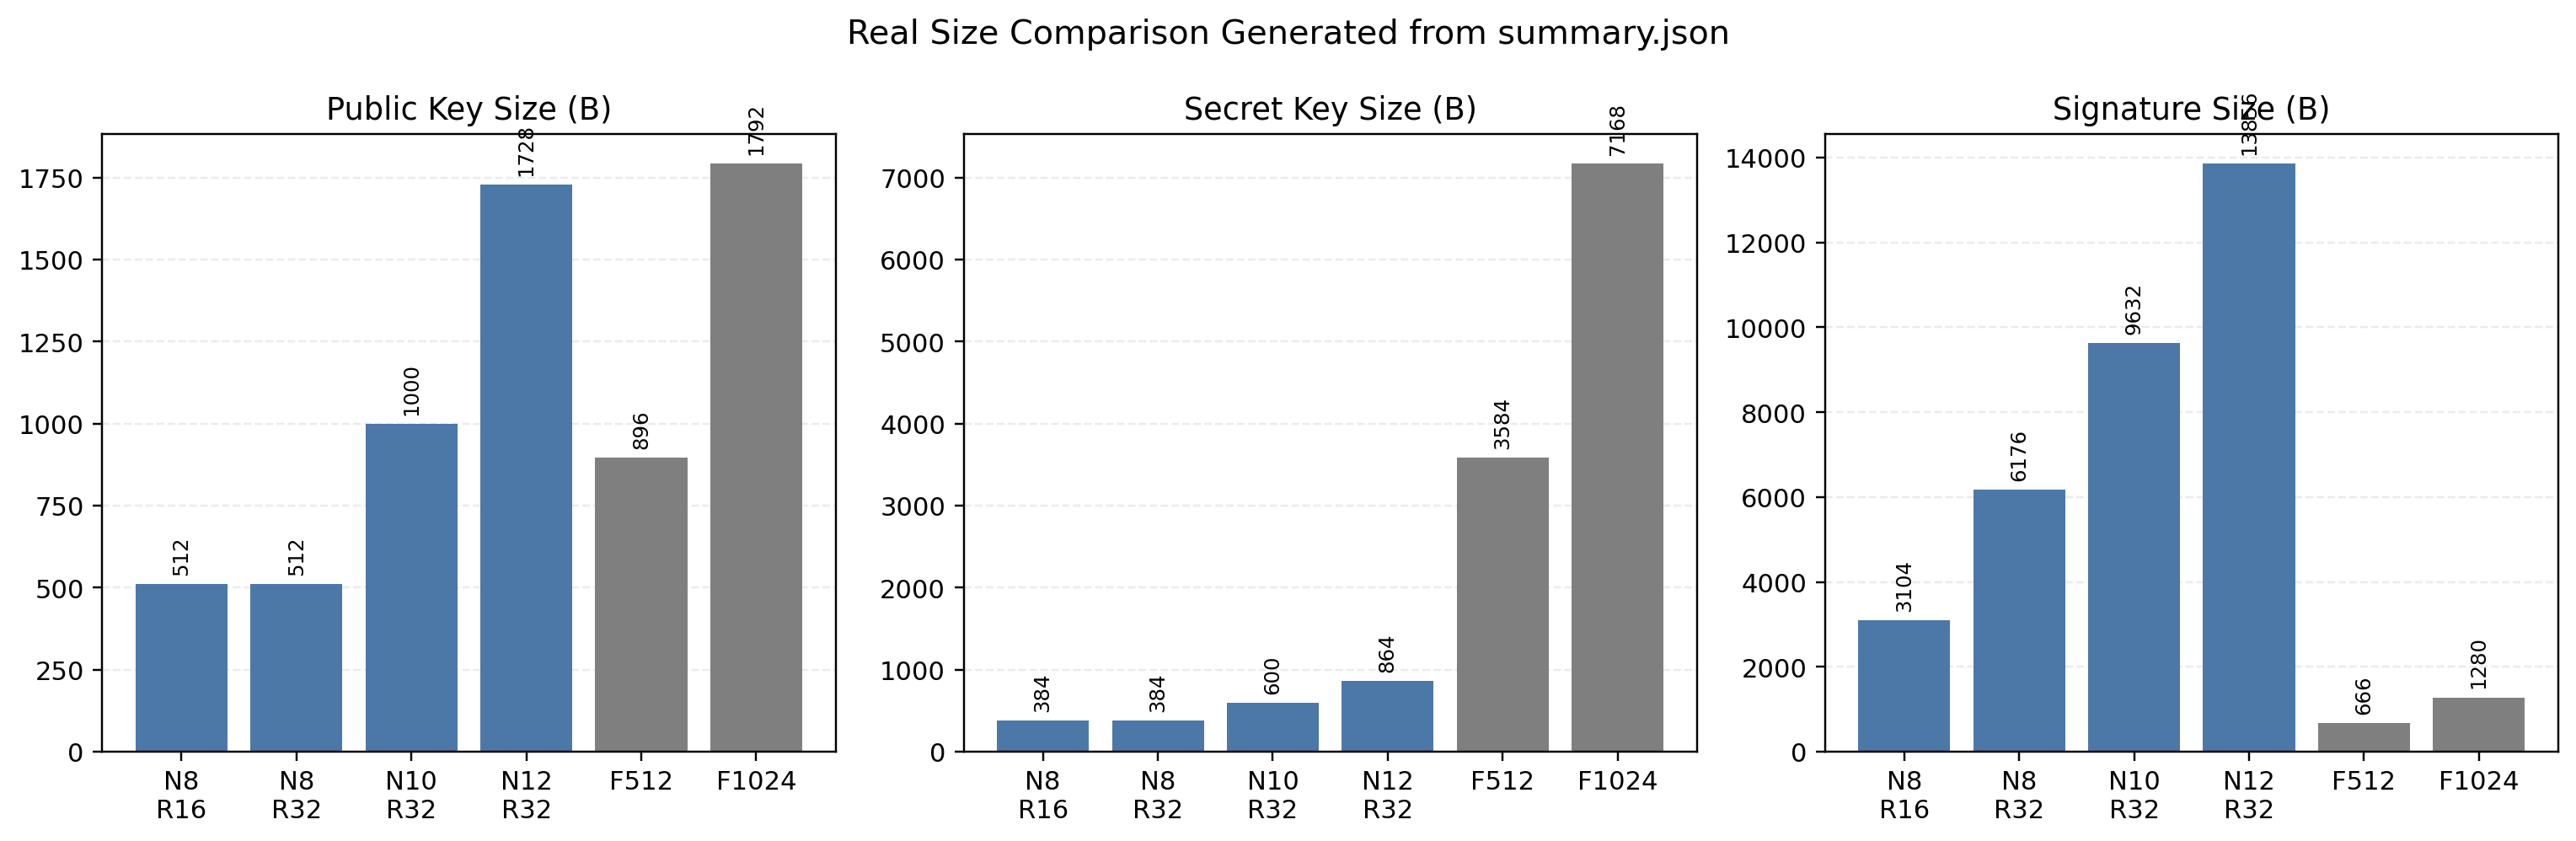
\includegraphics[width=\textwidth]{../experiments/results/size_comparison.png}
    \caption{基于真实运行结果自动生成的 TITAN 与 Falcon 尺寸开销对比图}
\end{figure}

由表 2 可得到如下可量化结论：
\begin{itemize}
    \item 在本机实验中，TITAN 的 \textbf{密钥生成时间显著低于} Falcon。以 $N=8$、rounds=16 的 TITAN 参数点为例，其 KeyGen 均值为 4.539 ms；相比 Falcon-512 的 2328.044 ms，约快 512.9 倍。这意味着在节点准入控制器或设备侧批量灌装阶段重新生成测试密钥、轮换样机密钥时，初始化等待成本更低。
    \item 在本机实验中，TITAN 的 \textbf{验证延迟显著低于} Falcon。以 TITAN N=8、rounds=16 为例，其 Verify 均值为 1.808 ms，相比 Falcon-512 的 4.263 ms 约快 2.36 倍；对应验证吞吐量约为 553.097 次/秒，更适合高并发节点接入控制器或高频 V2X 广播入口对消息做快速放行或阻断。
    \item 在公钥维度上，TITAN 可取得较紧凑表示。以 TITAN N=8、rounds=16 为例，其公钥为 512 字节，仅为 Falcon-512 公钥 896 字节的约 57\%；以 TITAN N=12、rounds=32 为例，其公钥 1728 字节略低于 Falcon-1024 的 1792 字节，这有利于在设备证书区、启动链元数据区和模型清单头部中嵌入公钥或其索引。
    \item 当前未压缩原型实现下，TITAN 的 \textbf{签名字节数明显大于} Falcon。例如 TITAN N=8、rounds=16 的签名为 3104 字节，为 Falcon-512 的约 4.66 倍；这表明本申请在验证时延和部署路径上有优势，但在固件包头、模型清单和网络控制报文中的签名压缩方面仍存在明确优化空间。
\end{itemize}

将表 2 中的真实测量数据映射到六类典型部署入口，可得到更直接的工程证据：其一，若将 TITAN N=8、rounds=16 用于节点准入控制器，则单次验证均值为 1.808 ms、P95 为 2.674 ms，连续处理 100 个节点认证报文约需 180.8 ms，连续处理 1000 个节点认证报文约需 1.808 s；其二，若将 TITAN N=10、rounds=32 用于固件升级代理，则单次验证均值为 4.136 ms、P95 为 5.343 ms，连续校验 1000 份固件升级清单约需 4.136 s；其三，若将 TITAN N=12、rounds=32 用于模型发布校验代理，则单次验证均值为 4.806 ms、P95 为 6.271 ms，连续校验 1000 份模型发布清单约需 4.806 s；其四，若将联邦学习梯度载荷映射到同样的张量验签算子，则可在 GPU/NPU 侧利用相同重构逻辑完成来源校验，并在显存内部直接决定是否放行进入聚合函数，从而减少显存到 CPU 的往返搬运；其五，若将分布式训练中的梯度分片、参数块或检查点分片映射到同样的张量验签算子，则可在同步代理或训练框架运行时中快速完成来源校验，减少异常分片进入 all-reduce 和断点恢复流程；其六，若将 V2X 广播载荷映射到同样的验签流程，则 1 到 5 ms 量级的验证预算足以支持车端对高频广播消息进行入口拦截。换句话说，在消息进入规划链路前，系统就有机会把异常广播拦住。上述具体毫秒数值直接来自 \path{experiments/results/summary.json} 的真实测量结果；联邦学习、分布式训练同步和 V2X 场景中的工程分析，是基于相同验签算子、相同测量时延和相同硬件映射逻辑所作的工程推导，不是新增编造的现场测试数据。

\textbf{参数变化时的时间与尺寸趋势}

\begin{table}[htbp]
    \centering
    \small
    \resizebox{\textwidth}{!}{%
    \begin{tabular}{|l|c|c|c|c|c|c|}
        \hline
        TITAN参数点 & $N$ & rounds & 公钥字节数 & 签名字节数 & Sign均值(ms) & Verify均值(ms) \\
        \hline
        TITAN N=8, rounds=16 & 8 & 16 & 512 & 3104 & 16.534 & 1.808 \\
        \hline
        TITAN N=8, rounds=32 & 8 & 32 & 512 & 6176 & 33.794 & 3.495 \\
        \hline
        TITAN N=10, rounds=32 & 10 & 32 & 1000 & 9632 & 43.297 & 4.136 \\
        \hline
        TITAN N=12, rounds=32 & 12 & 32 & 1728 & 13856 & 50.150 & 4.806 \\
        \hline
    \end{tabular}}
    \caption{TITAN 参数扩展下的真实测量结果}
\end{table}

由表 3 可见，本申请的参数变化趋势具备良好的可解释性：
\begin{itemize}
    \item 当维度固定为 $N=8$、将 rounds 从 16 增加到 32 时，签名字节数由 3104 字节增加到 6176 字节，约增长 1.99 倍；签名时间由 16.534 ms 增加到 33.794 ms，约增长 2.04 倍；验证时间由 1.808 ms 增加到 3.495 ms，约增长 1.93 倍，表明 rounds 的影响接近线性。
    \item 当 rounds 固定为 32、将维度从 $N=8$ 提高到 $N=12$ 时，公钥由 512 字节增加到 1728 字节，约增长 3.38 倍；签名时间由 33.794 ms 增加到 50.150 ms，约增长 1.48 倍；验证时间由 3.495 ms 增加到 4.806 ms，约增长 1.38 倍，说明参数增长趋势平稳、可预测。
    \item 以 TITAN N=12、rounds=32 为例，公钥为 1728 字节，略低于 Falcon-1024 的 1792 字节；验证时间为 4.806 ms，约为 Falcon-1024 的 44.9\%，显示出本申请在较大参数点下仍具有较好的验证效率优势。
\end{itemize}

综上，真实试验结果表明：本申请方案在当前原型实现中，已经能够以可复现方式说明其稳定运行能力、篡改拒绝能力以及工程时间和尺寸成本特征。其当前最明确的工程优势集中在：\textbf{更快的密钥生成、更快的验证路径、较小的公钥表示}；其当前最明确的工程代价则是：\textbf{未压缩签名尺寸较大}。因此，该组数据既支撑了本申请的创新可实现性，也为后续进一步的签名压缩和参数优化提供了量化依据。

\textbf{上述真实数据的证明范围}

上述真实数据已经直接证明：其一，本申请给出的 TITAN 算法流程能够在本地代码中完成密钥生成、签名生成、签名验证以及篡改拒绝，且在当前执行的 200 次 TITAN 验证试验中未观察到失败样本；其二，本申请在同一机器、同一运行环境下，相较本地 Falcon 参考实现，已经展示出更快的密钥生成路径和更快的验证路径；其三，本申请当前原型在公钥尺寸方面具备一定优势，但在未压缩签名尺寸方面仍有明显优化空间。上述真实数据尚未直接证明的内容包括：与 NIST 标准参数逐点对齐的安全等级结论、针对大规模密码分析的最终安全性结论、以及经过专门常数时间实现与物理测试验证后的最终侧信道强度结论。因此，本申请将该组实验明确定位为\textbf{真实性能与可实现性证据}，不将其表述为已经完成全部标准化安全论证，从而准确区分已被数据支撑的内容与后续仍需继续论证的内容。

\subsection{扩展实施方式}

除上述基本实施方式外，本申请还包括如下扩展方式：

\begin{itemize}
    \item 可将三阶张量扩展为四阶或更高阶张量，以构造更多模态上的联合陷门；
    \item 可将二元挑战扩展为多元挑战，以减少在相同安全目标下的总轮数；
    \item 可采用种子展开的随机矩阵生成方式，降低私钥和签名中的响应存储量；
    \item 可将张量按切片方式进行并行调度，以适配 GPU/NPU 的批量矩阵乘法接口；
    \item 可将本申请的方法封装为签名服务器、密码卡、可信模组、终端 SoC 固件、模型发布校验代理、联邦学习训练框架插件、分布式训练同步插件、车端 V2X 验签模块或云端签名服务。
\end{itemize}

\subsection{六类重点应用场景说明}

为最大化本申请作为技术方案的客体稳定性，本申请优先强调以下六类具有物理属性、硬件边界和可量化技术效果的应用场景：

\begin{itemize}
    \item \textbf{量子计算网络节点认证场景}：验签动作发生在节点准入控制器，目标是在节点接入前完成证书摘要和角色字段的真实性校验，技术效果体现为减少错误节点接入与提升控制面放行效率。举例来说，一个量子计算任务调度平台在给新节点分配量子比特资源前，先校验该节点上报的身份摘要和角色标签是否被合法签名，签名不通过则不允许接入。该场景中本专利特别重要，因为节点认证是整个系统的入口，一旦入口被放过，后续所有协同计算都会受影响。
    \item \textbf{AI 加速设备固件升级场景}：验签动作发生在可信启动链或升级代理，目标是在镜像装载前校验版本、哈希和回滚计数器，技术效果体现为阻断回退镜像和减少设备侧专用密码协处理器依赖。举例来说，一块训练卡在升级固件前，系统先检查升级包里的设备型号、固件版本号和镜像哈希，只有签名和版本都正确时才允许装载。该场景中本专利特别重要，因为固件一旦装错，影响通常不是单次失败，而是整块设备的可用性和稳定性。
    \item \textbf{模型发布完整性校验场景}：验签动作发生在模型仓库校验代理，目标是在模型下载、加载或分发前校验权重摘要和依赖摘要，技术效果体现为减少污染模型进入推理环境的概率。举例来说，模型仓库在把一个大模型推送到推理集群前，先检查模型文件摘要、依赖包摘要和目标加速器型号是否与签名一致，不一致则停止发布。该场景中本专利特别重要，因为模型发布通常是一次发布、多处使用，前端没拦住，后端影响范围会很大。
    \item \textbf{跨域联邦学习梯度防投毒场景}：验签动作发生在 GPU/NPU 显存侧或训练框架计算图内部，目标是在模型聚合前校验梯度张量或模型更新块的来源合法性和完整性，技术效果体现为减少 PCIe 或其它主机总线搬运开销、提高集群吞吐量并降低 CPU 参与度。进一步地，本申请可将验签逻辑编译为深度学习框架自定义算子，在显存内部完成原生验签和异常梯度阻断。举例来说，医院 A、医院 B 和研究机构 C 共同训练一个医学影像模型时，聚合节点在接收每一轮梯度更新后，先在显存里检查该更新是否来自合法参与方、是否被篡改，校验不通过则该梯度不会进入聚合。该场景中本专利特别重要，因为联邦学习训练轮次多、梯度量大，若每轮都先搬运再验签，系统开销会被持续放大。
    \item \textbf{分布式 AI 训练集群中的梯度/检查点同步验签场景}：验签动作发生在训练框架同步代理、分布式训练运行时或加速卡通信侧，目标是在梯度分片、参数块和检查点分片进入同步链路前完成来源合法性和完整性校验，技术效果体现为减少异常数据进入 all-reduce、参数恢复和断点续训流程，并尽量复用现有张量算力。举例来说，多机多卡训练一个大模型时，节点在同步梯度分片和 checkpoint 分片之前，先检查分片摘要、训练步号和作业标识是否与签名一致，不一致则不允许进入同步流程。再例如，训练任务在故障后需要从最近一次 checkpoint 恢复时，系统也可以先校验检查点分片来源是否可信，再决定是否恢复。该场景中本专利特别重要，因为训练集群同步频率高、数据量大，只要同步链路里混入异常分片，就可能拖垮整轮训练或污染恢复过程。
    \item \textbf{自动驾驶与车路协同 V2X 高频广播验签场景}：验签动作发生在车端通信控制器、车载 AI 芯片或路侧消息接收模块，目标是在广播消息进入感知融合、预测或轨迹规划链路前完成真实性校验，技术效果体现为降低伪造广播进入车辆控制决策的概率，并满足毫秒级处理预算。举例来说，车辆每隔数十毫秒接收周边车辆的位置、速度和刹车意图广播，车端先检查消息时间戳、发送方标识、位置字段和事件标签是否与签名一致，校验通过后再交给规划模块。该场景中本专利特别重要，因为 V2X 消息更新快、决策链路短，一旦假消息进入后续模块，风险会直接反映到车辆的物理动作上。
\end{itemize}

%==============================================================================
\section{本申请提案的关键点和欲保护点}
%==============================================================================

本申请提出主要包含以下创新点和保护点：

(1) \textbf{基于三模态张量同构关系构造公私钥陷门}：以公开基准张量 $\mathcal{T}_0$ 为参照，通过三个私钥可逆矩阵在不同模态上的联合作用得到公钥张量 $\mathcal{T}_{pk}$，区别于现有格、哈希、码或传统多变量签名的线性/低阶结构。

(2) \textbf{基于双视图一致性的零知识签名机制}：在同一承诺张量下，允许验证端针对不同挑战分别使用 $\mathcal{T}_0$ 或 $\mathcal{T}_{pk}$ 完成重构，从而形成适合 Fiat-Shamir 变换的签名结构。

(3) \textbf{不依赖噪声采样的有限域签名实现路径}：签名和验证仅需有限域矩阵乘法、求逆和张量收缩，更易形成常数时间实现，不依赖高斯采样、拒绝采样或浮点近似。

(4) \textbf{结构化业务载荷与验证入口一体化设计}：将节点身份证书摘要、节点角色与调度域字段、固件版本与回滚计数器、模型权重哈希与依赖清单摘要、联邦学习梯度元数据、训练同步分片元数据以及 V2X 广播字段纳入原生签名对象，并限定其分别在节点准入控制器、可信启动/升级代理、模型仓库校验代理、联邦学习聚合运行时、训练同步代理和车端消息入口处触发验证，从而使技术方案与具体场景不可分割。

(5) \textbf{适配张量加速硬件的场景化密码原语设计}：将签名核心运算直接表达为张量收缩与矩阵乘法，使其能够复用 AI 芯片、GPU、NPU 或张量核心的并行计算能力，特别适合节点控制面批量验签、设备升级批量校验、模型分发批量校验、训练同步链路验签以及联邦学习显存内验签。

(6) \textbf{覆盖方法、系统、设备和介质的统一方案}：保护点不仅包括签名流程本身，还包括参数生成系统、验证设备、存储签名程序的计算机可读介质及其在六类物理场景中的部署结构。

%==============================================================================
\section{与第三条中最接近的现有技术相比，本申请提案有何技术优点}
%==============================================================================

与第三节中最接近的现有技术，尤其是基于格的紧凑型签名方案和通用识别到签名方案相比，本申请具有如下技术优点：

(1) \textbf{避免离散高斯采样和浮点路径}：本申请的核心流程建立在有限域矩阵和张量运算上，较格签名更易实现整数化、分支稳定的执行路径。

(2) \textbf{更适合常数时间与侧信道防护}：由于不存在高斯采样重试、浮点近似和范数拒绝过程，本申请更有利于构造功耗、缓存和时延表现更稳定的实现。

(3) \textbf{验证关系严格由代数抵消给出}：验证端通过公钥张量与隐身重构矩阵的模态抵消恢复承诺，签名正确性来源于显式代数关系，便于做形式化推导与实现自检。

(4) \textbf{与张量硬件天然对齐}：本申请的主要计算是矩阵乘法和张量收缩，能够直接映射到现有 AI 加速硬件的软件栈中，在批量签名、批量验证、边云协同验证、训练同步验签和联邦学习梯度验签场景中具有工程优势。

(5) \textbf{公钥表示紧凑且可结构化压缩}：在中等维度参数下，公钥可直接表示为有限域三阶张量；若进一步结合种子生成和结构化矩阵，还可继续压缩密钥分发成本。

(6) \textbf{技术路线区别于现有主流后量子路线}：本申请不依赖格噪声、Merkle 树、纠错码译码或椭圆曲线同源，而是采用高阶张量同构陷门作为核心困难结构，技术路径差异明显。

(7) \textbf{克服总线带宽瓶颈，实现显存内原生验签}：针对联邦学习等海量张量数据交互场景，本方案凭借签名的全张量化特征，可将验签逻辑嵌入训练框架计算流图，在显存内部完成验证并直接阻断异常梯度，从而减少 PCIe 或其它主机总线搬运开销，提升大规模高频校验场景下的系统吞吐量。

%==============================================================================
\section{其他有助于理解本申请提案的技术资料}
%==============================================================================

(1) \textbf{参数示例}：在一个示例实现中，可取 $p=251$、$N=10$、$r=32$。该参数仅用于说明本申请的基本可实现性，不构成对保护范围的限定。

(2) \textbf{软件验证示例}：可采用 Python、C/C++、Rust 或硬件描述语言实现本申请方案。软件实现中可使用爱因斯坦求和约定、批处理矩阵乘法或张量库来完成
\[
\mathcal{T} \times_1 A \times_2 B \times_3 C
\]
运算。

(3) \textbf{安全性理解}：本申请方案的安全性可理解为建立在如下问题的计算困难性之上：对于给定的公开基准张量 $\mathcal{T}_0$ 和公钥张量 $\mathcal{T}_{pk}$，在不知道私钥矩阵 $U,V,W$ 的情况下，难以恢复满足
\[
\mathcal{T}_{pk}=\mathcal{T}_0 \times_1 U \times_2 V \times_3 W
\]
的等价陷门结构，或难以同时回答多轮挑战并伪造一致签名。

(4) \textbf{适用场景}：本申请可应用于量子计算网络节点认证、模型文件签名、固件升级保护、分布式软件发布、跨域联邦学习梯度防投毒、分布式训练集群同步验签以及自动驾驶与车路协同 V2X 高频广播验签。

(5) \textbf{可替换部件}：哈希函数可选用 SHA-256、SHA3、SM3 或其它安全散列函数；有限域模数 $p$、张量阶数和矩阵结构均可按不同安全等级进行配置。

%==============================================================================
\section{本申请提案的侵权证据可获得性}
%==============================================================================

本申请提出的侵权证据具有较高的可获得性，主要包括：

(1) \textbf{公钥格式证据}：若被控产品或系统公开输出以三阶张量为主体的公钥、证书或设备身份数据，并公开声明其由公开基准张量经三组可逆矩阵作用生成，则可据此识别是否采用了本申请的核心公钥结构。

(2) \textbf{签名格式证据}：若签名数据中包含基于消息与多轮承诺导出的摘要以及按挑战位选择输出的三组矩阵响应，则可据此判断其是否落入本申请的签名格式和应答机制。

(3) \textbf{验证逻辑证据}：若被控实现中同时存在“使用公开基准张量验证第一类响应”和“使用公钥张量验证第二类响应”的双路径验证逻辑，则可作为侵权判定的重要技术证据。

(4) \textbf{程序和固件证据}：通过对软件二进制、固件、驱动、密码模块接口或加速内核进行逆向分析，如发现有限域矩阵求逆、模态张量乘法和基于哈希挑战的双分支验证流程，可作为实施本申请技术方案的证据。

(5) \textbf{部署和接口证据}：在云签名服务、芯片 SDK、可信模组 API、模型发布校验代理接口、联邦学习框架插件、训练同步代理接口、车端 V2X 验签日志、设备升级日志或调试接口中，如公开暴露与张量维度、域参数、模态乘法、轮次挑战等对应的调用参数，也可作为辅助证据。

\end{document}
